\documentclass[11 pt]{book}
\usepackage[utf8]{inputenc}
\usepackage[spanish]{babel}
\usepackage{graphicx}
\usepackage[margin=2.5cm]{geometry}
\begin{document}
\title{\textbf {\Huge Memoria del proyecto Polis}}
\author{
	\textbf {Ingeniería del Software de Gestión II - Grupo 10 - Versión documento: 3.0}\\\\
	Samuel Navas Portillo\\
	Juan Jesús Pérez Luna\\
	Manuel de los Santos Campos\\
	María José Sancha Maya\\
	Ángel Martínez Olivares\\
	José Antonio Jiménez Carmona}
\maketitle
\tableofcontents{}

\chapter{Vídeo explicativo del juego}
	El siguiente vídeo online explica brevemente cómo se juega al juego de mesa Polis.\\ \\
	\texttt{http://www.youtube.com/watch?v=gTCdMBfJiHo}
	
\chapter{Planificación Temporal}
	En una primera conversación del grupo realizada el 29 de Septiembre, se llega al siguiente acuerdo sobre la planificación de las reuniones regulares del grupo y de las distintas entregas del proyecto:\\

    \section*{Reuniones ordinarias}
	Cada martes de 9:30 a 11:30 y/o viernes de 12:30 a 14:30 de cada semana hasta que tenga lugar la última entrega del proyecto, el grupo debe reunirse para analizar el estado del proyecto y del grupo y, en su caso, discutir y tomar las decisiones que e tomen oportunas.\\

    \section*{Entregas de las iteraciones}
	La primera entrega del proyecto será el día 7 de Octubre de 2010. Las siguientes entregas (2ª y 3ª Iteración) serán, respectivamente, los días 14 de Octubre y 11 de noviembre respectivamente.

	\section*{Reuniones extraordinarias}
		El martes 5 de Octubre (de 17:30 a 20:30) y el miércoles 6 de Octubre (de 9:00 a 11:30, de 15:30 a 17:30 y de 19:30 a 21:30) tuvimos 2 reuniones extra respectivamente.

\chapter{Seguimiento}
	Este capítulo presenta las actividades concretas realizadas por cada miembro del grupo así como su tiempo invertido.
	
	\section*{Actividades}
		\begin{itemize}
			\item \textbf {Samuel Navas Portillo}
				\begin{enumerate}
					\item Búsqueda de materiales: 1h 30min
					\item Fabricación de las fichas y cartas del juego: 2h
					\item Lectura de las Normas: 1h
					\item Impresión de las Normas del juego: 1h 30min
					\item Simulación de partidas: 2h
					\item Guión del vídeo (1ª parte): 2h
					\item Guión del vídeo (2ª parte): 2h
					\item Estudio/repaso del tema de análisis de Ingeniería del Software de Gestión 1 y propuesta de diseño UML: 10h
					\item Diseño del diagrama UML de análisis, diseño del diagrama UML de diseño, implementación de parte del proyecto (código), asignación de responsabilidades e implantación de Eclipse y Subversion: 8h
				\end{enumerate}
			\item \textbf {Juan Jesús Pérez Luna}
				\begin{enumerate}
					\item Análisis y síntesis de las Normas del juego: 3h
					\item Impresión del juego: 30min
					\item Fabricación de las fichas y cartas del juego: 2h
					\item Lectura de las Normas: 1h
					\item Simulación de partidas: 2h
					\item Guión del vídeo y actor (mano) (1ª parte): 2h
					\item Guión del vídeo (2ª parte): 1h
					\item Estudio/repaso del tema de análisis de Ingeniería del Software de Gestión 1 y propuesta de diseño UML: 10h
					\item Diseño del diagrama UML de análisis, diseño del diagrama UML de diseño, diseño de la estructura del código fuente del proyecto, implementación de parte del proyecto (código), asignación de responsabilidades e implantación de Eclipse y Subversion: 10h
				\end{enumerate}
			\item \textbf {Manuel de los Santos Campos}
				\begin{enumerate}
					\item Lectura de las Normas: 2h
					\item Simulación de partidas: 2h
					\item Guión del vídeo (1ª parte): 2h
					\item Guión del vídeo y actor (mano) (2ª parte): 2h
					\item Estudio/repaso del tema de análisis de Ingeniería del Software de Gestión 1 y propuesta de diseño UML: 10h
					\item Implantación de Eclipse y Subversion y asignación de responsabilidades: 5h
				\end{enumerate}
			\item \textbf {María José Sancha Maya}
				\begin{enumerate}
					\item Búsqueda y preparación del equipo de grabación del video: 30min
					\item Fabricación tablero: 2h
					\item Lectura de las Normas: 1h
					\item Simulación de partidas: 2h
					\item Guión del vídeo (1ª parte): 2h
					\item Grabación del vídeo (cámara): 2h
					\item Edición del vídeo (postproducción): 5h
					\item Estudio/repaso del tema de análisis de Ingeniería del Software de Gestión 1 y propuesta de diseño UML: 10h
					\item Implantación de Eclipse y Subversion y traducciones: 4h
				\end{enumerate}
			\item \textbf {Ángel Martínez Olivares}
				\begin{enumerate}
					\item Búsqueda de materiales: 1h 30min
					\item Fabricación de las fichas y cartas del juego: 2h
					\item Lectura de las Normas: 1h
					\item Simulación de partidas: 2h
					\item Guión del vídeo y actor (voz) (1ª parte): 2h
					\item Guión del vídeo y actor (voz) (2ª parte): 3h
					\item Estudio/repaso del tema de análisis de Ingeniería del Software de Gestión 1 y propuesta de diseño UML: 10h
					\item Implantación de Eclipse y Subversion y asignación de responsabilidades: 5h
				\end{enumerate}
			\item \textbf {José Antonio Jiménez Carmona}
				\begin{enumerate}
					\item Impresión del juego: 30min
					\item Fabricación de las fichas y cartas del juego: 2h
					\item Lectura de las Normas: 1h
					\item Simulación de partidas: 1h 30min
					\item Guión del video (1ª parte): 2h
					\item Aprendizaje básico de "Latex" y producción de la Memoria (versión 1.0): 4h
					\item Estudio/repaso del tema de análisis de Ingeniería del Software de Gestión 1 y realización de Memoria: 10h
					\item Diseño del diagrama UML de diseño, implantación de Eclipse y Subversion y ampliación de la Memoria: 6h
				\end{enumerate}
		\end{itemize}

	\section*{Resumen de tiempo invertido y puntuaciones}
		Se presenta el total de horas de trabajo invertidas por cada miembro del grupo y la puntuación de esta iteración para cada miembro del grupo resultante de su esfuerzo individual (puntos repartidos entre los 6 miembros de 30 a repartir).\\
			
		\begin{tabular}{|c|c|c|}
			\hline
			Nombre & Tiempo total de iteraciones & Puntuación iteración actual\\
			\hline
			Samuel Navas Portillo & 30h & 6\\
			Juan Jesús Pérez Luna & 31h 30min & 8\\
			Manuel de los Santos Campos & 23h & 4\\
			María José Sancha Maya & 28h 30min & 4\\
			Ángel Martínez Olivares & 26h 30min & 4\\
			José Antonio Jiménez Carmona & 27h & 4\\
			\hline
		\end{tabular}
\chapter{Diagrama UML de Análisis}
	\begin{center}
		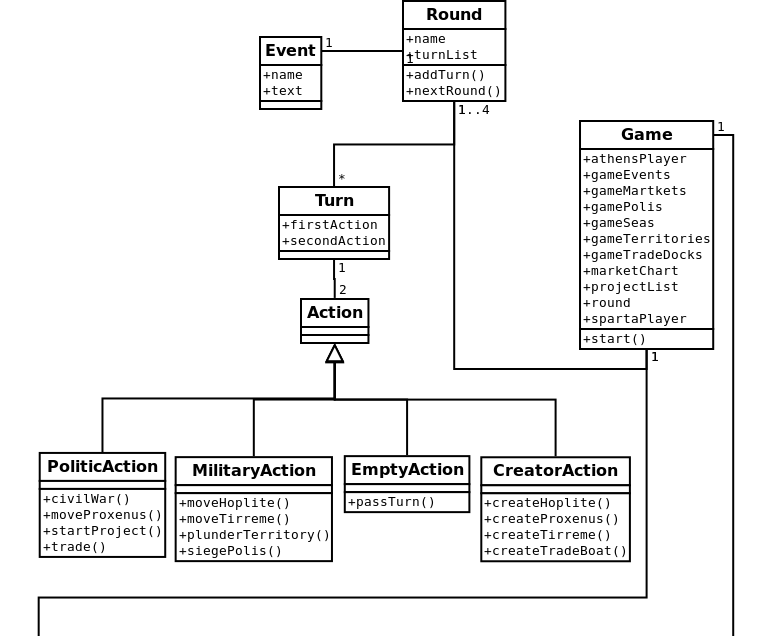
\includegraphics[width=500px]{analysis-uml/analysis-uml-part1.png}
		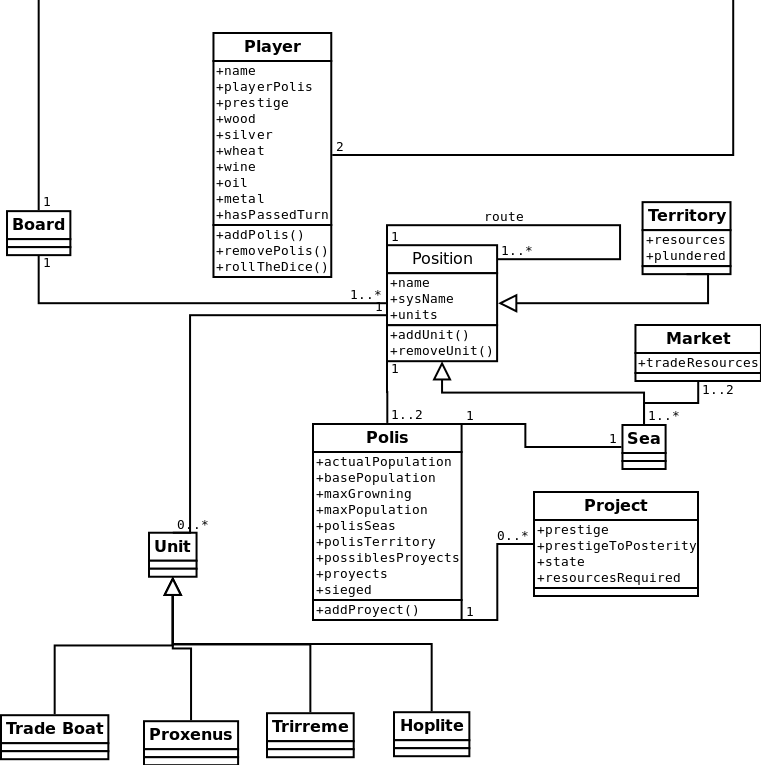
\includegraphics[width=500px]{analysis-uml/analysis-uml-part2.png}
	\end{center}
	
\chapter{Asignación de Responsabilidades}
    Nota: Hemos considerado como IU cuando no sólo llama directamente a un método de interfaz para comunicarse con el usuario, sino también cuando es el método que en su interior llamará al método concreto de interfaz de usuario.

    \begin{center}
        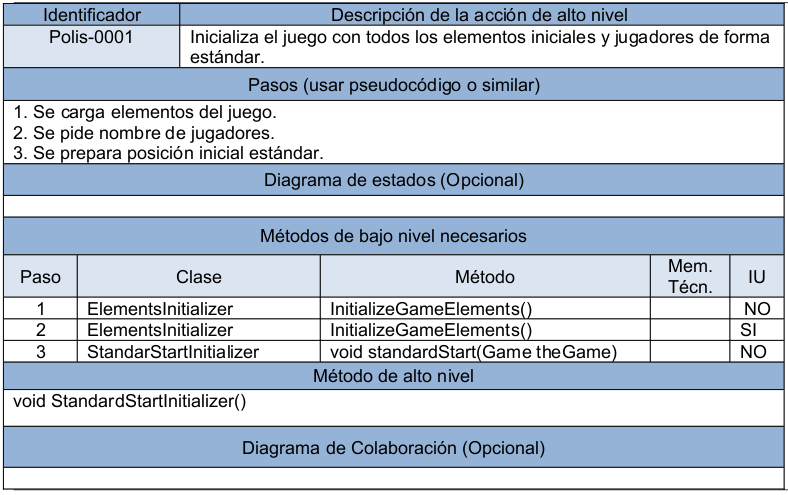
\includegraphics[width=500px]{responsabilities-allocation/polis-0001.png}
        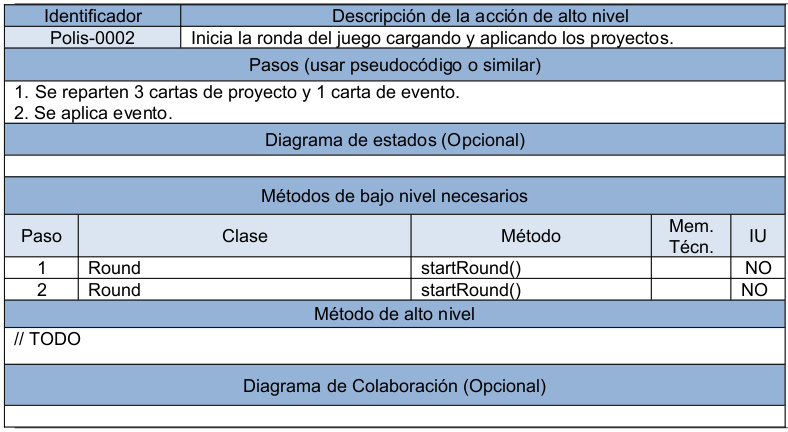
\includegraphics[width=500px]{responsabilities-allocation/polis-0002.png}
        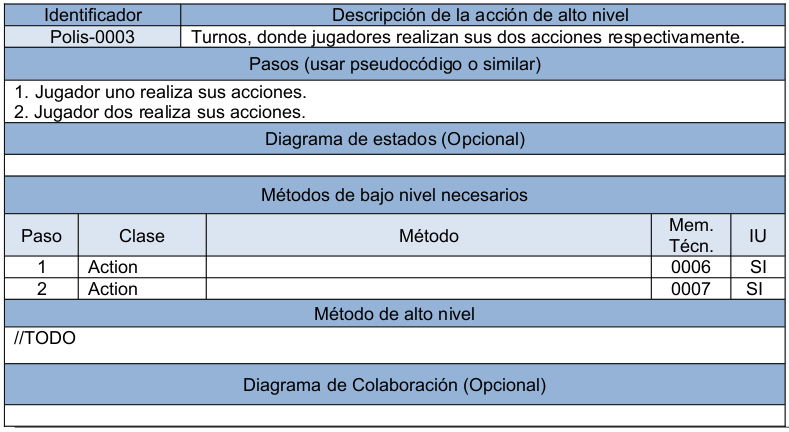
\includegraphics[width=500px]{responsabilities-allocation/polis-0003.png}
        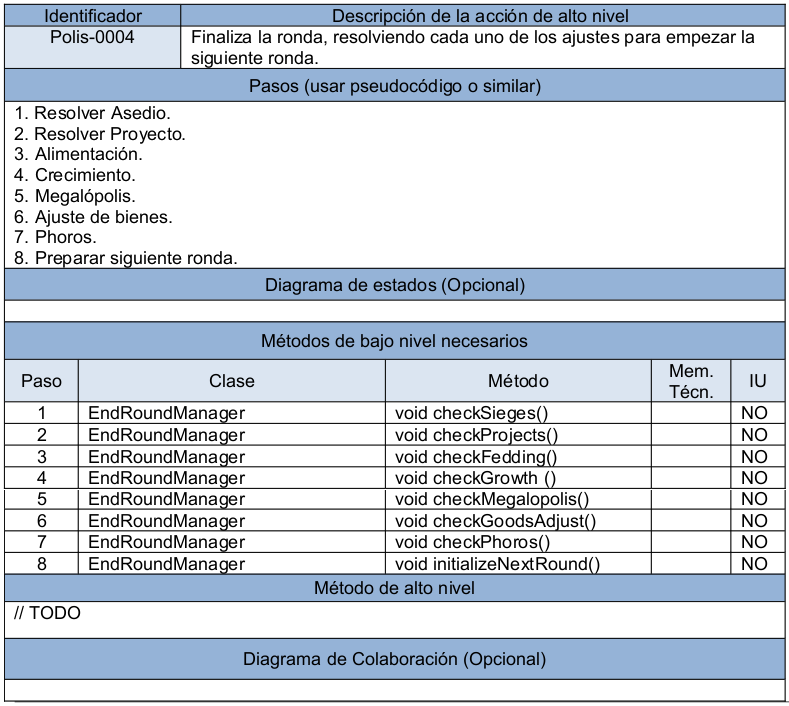
\includegraphics[width=500px]{responsabilities-allocation/polis-0004.png}
        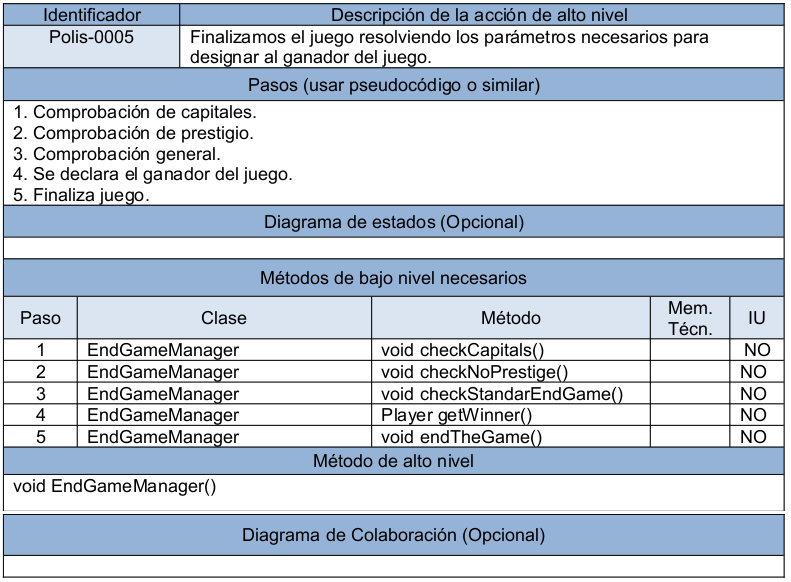
\includegraphics[width=500px]{responsabilities-allocation/polis-0005.png}
        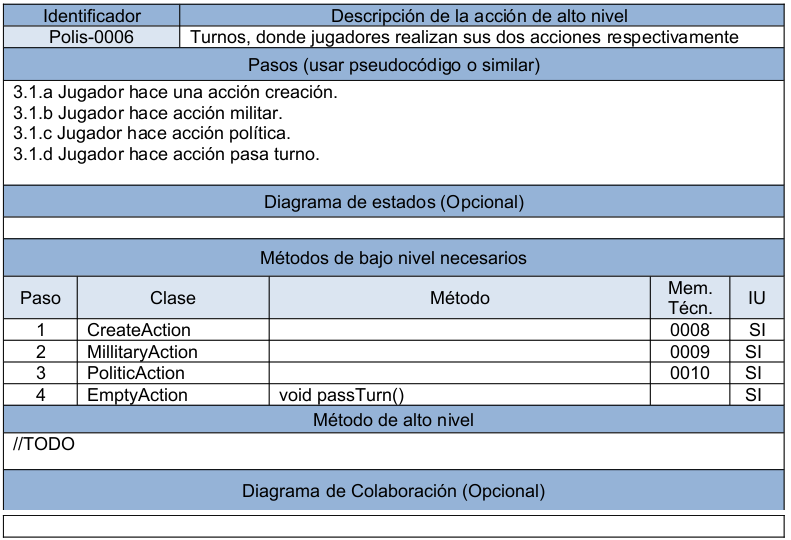
\includegraphics[width=500px]{responsabilities-allocation/polis-0006.png}
        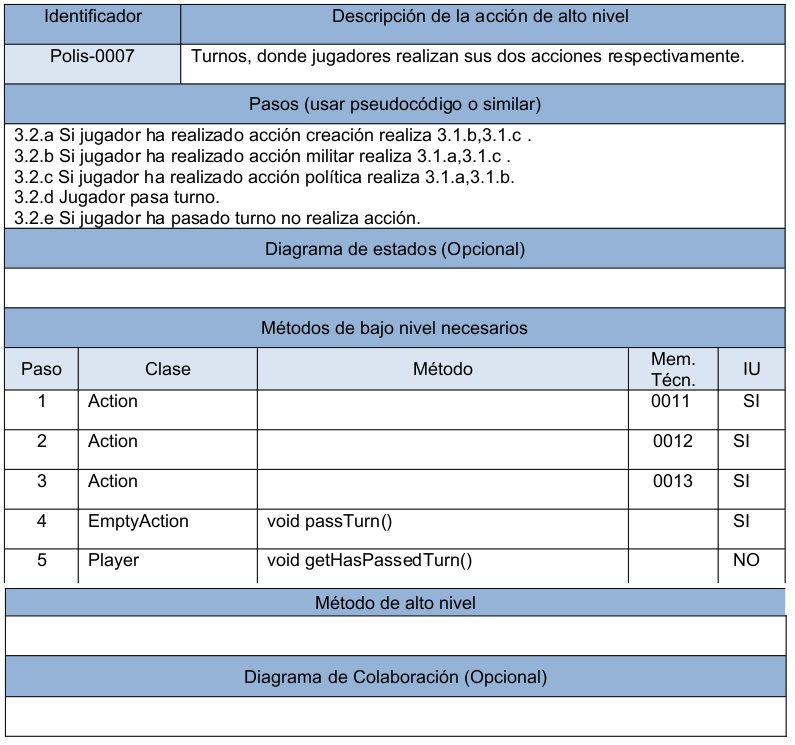
\includegraphics[width=500px]{responsabilities-allocation/polis-0007.png}
        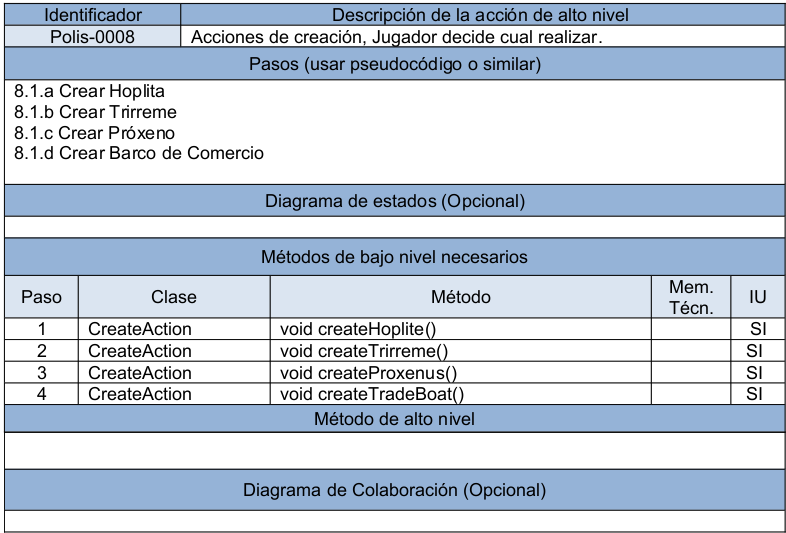
\includegraphics[width=500px]{responsabilities-allocation/polis-0008.png}
        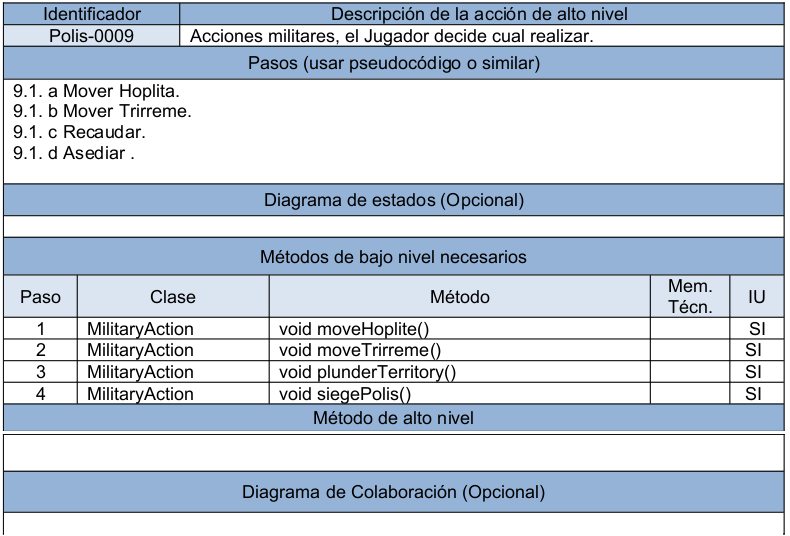
\includegraphics[width=500px]{responsabilities-allocation/polis-0009.png}
        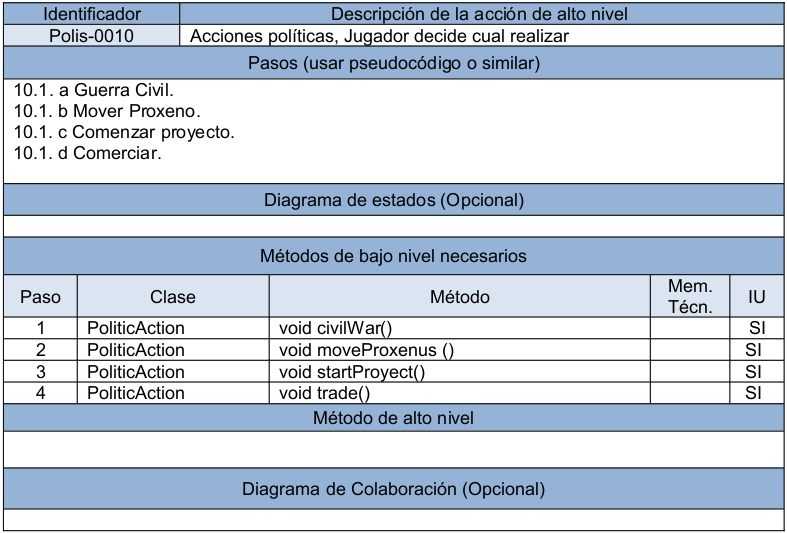
\includegraphics[width=500px]{responsabilities-allocation/polis-0010.png}
        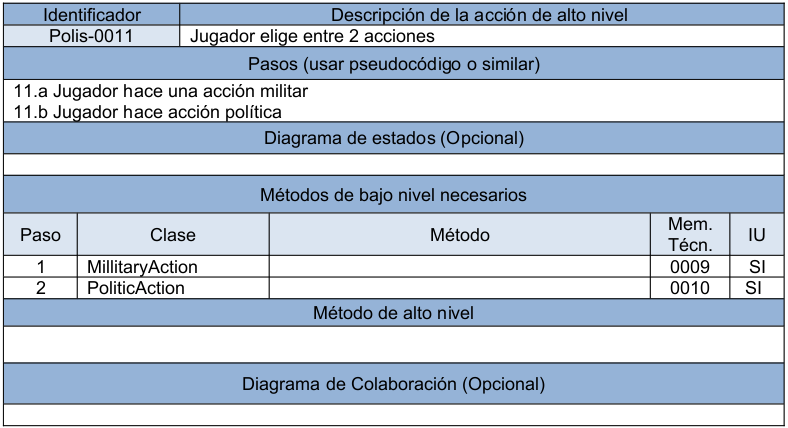
\includegraphics[width=500px]{responsabilities-allocation/polis-0011.png}
        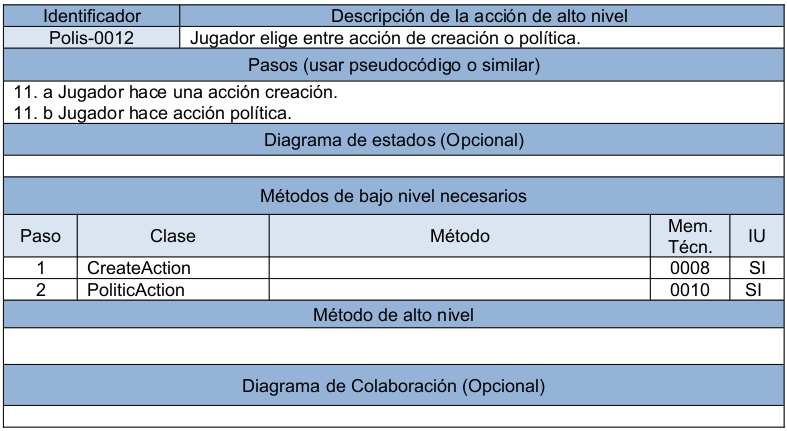
\includegraphics[width=500px]{responsabilities-allocation/polis-0012.png}
        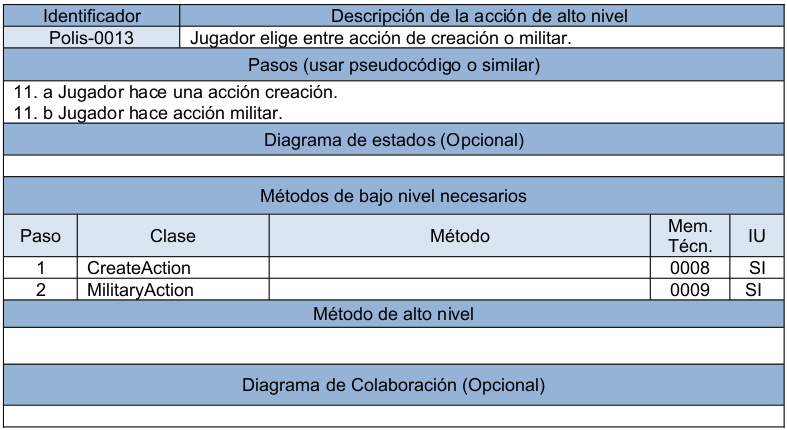
\includegraphics[width=500px]{responsabilities-allocation/polis-0013.png}
    \end{center}
\chapter{Diagrama UML de Diseño}
    \begin{center}
        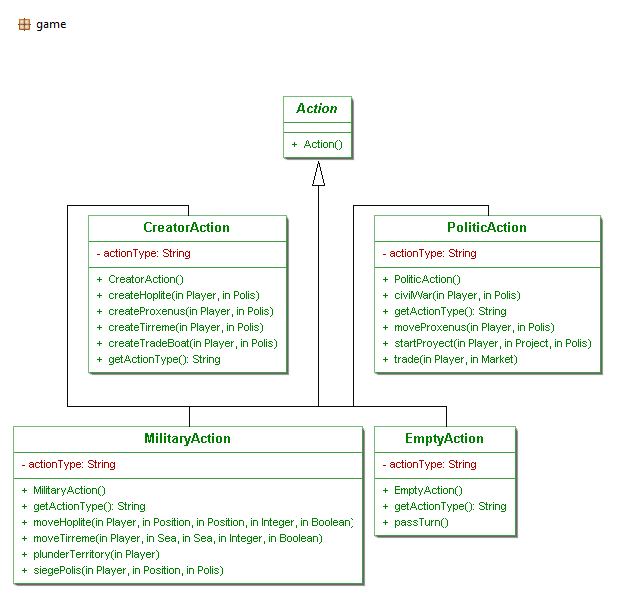
\includegraphics[width=500px]{design-uml/game-actions.png}
        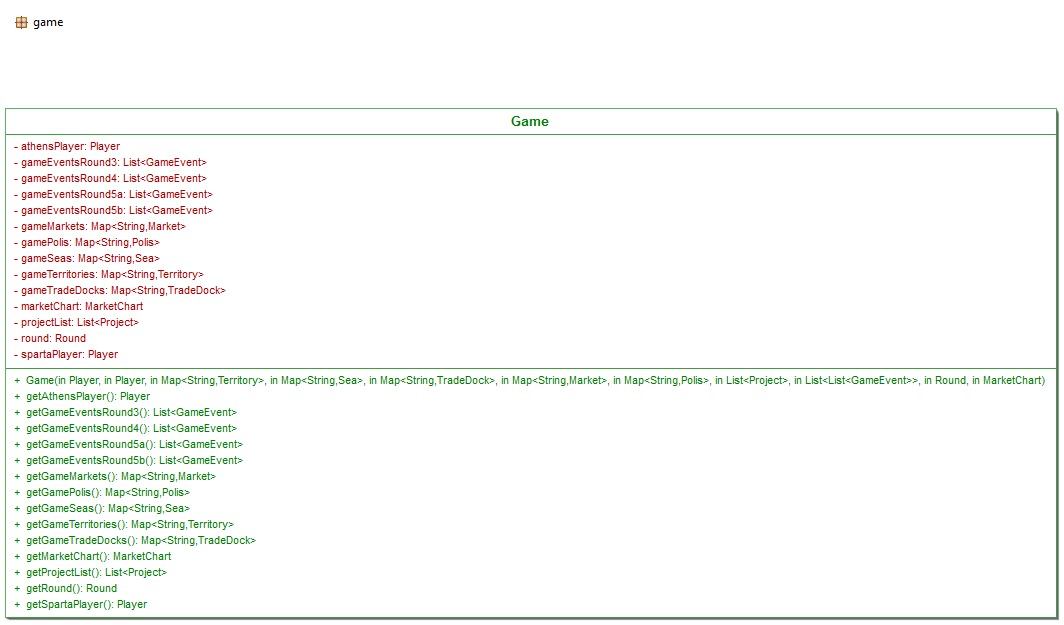
\includegraphics[width=500px]{design-uml/game-game.png}
        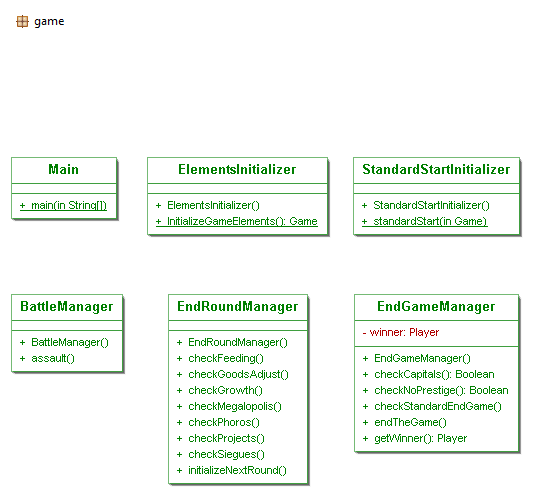
\includegraphics[width=500px]{design-uml/game-main-managers.png}
        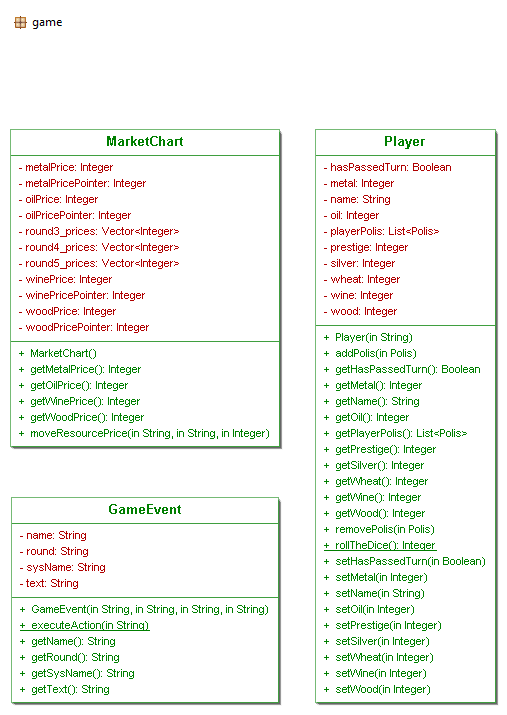
\includegraphics[width=500px]{design-uml/game-martket-gameevent-player.png}
        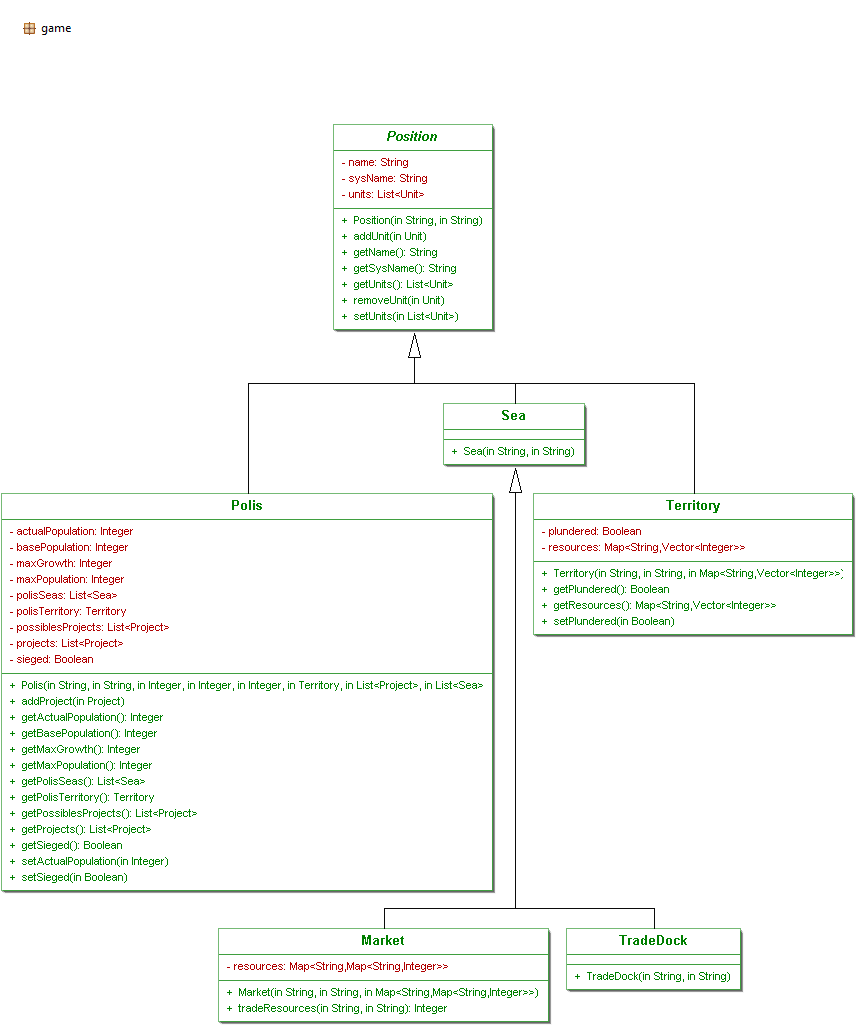
\includegraphics[width=500px]{design-uml/game-positions.png}
        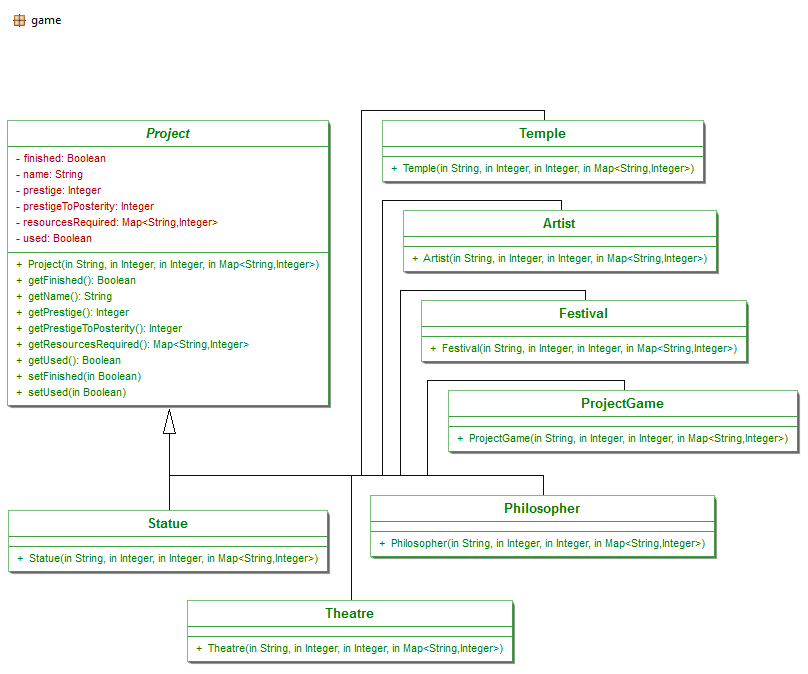
\includegraphics[width=500px]{design-uml/game-projects.png}
        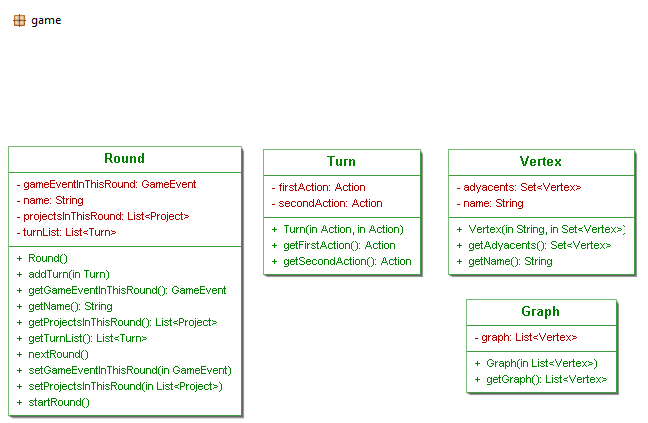
\includegraphics[width=500px]{design-uml/game-round-turn-graph-vertex.png}
        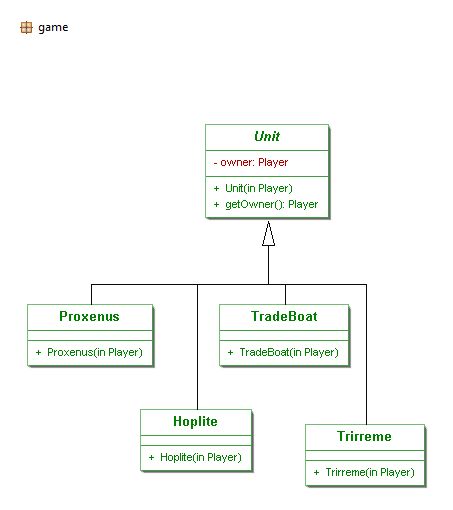
\includegraphics[width=500px]{design-uml/game-units.png}
        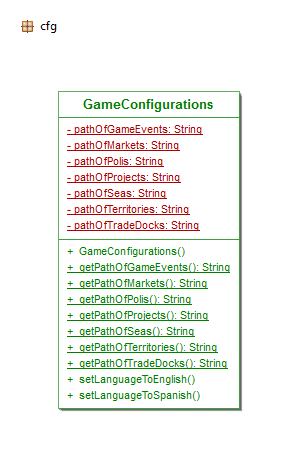
\includegraphics[width=500px]{design-uml/package-cfg.png}
        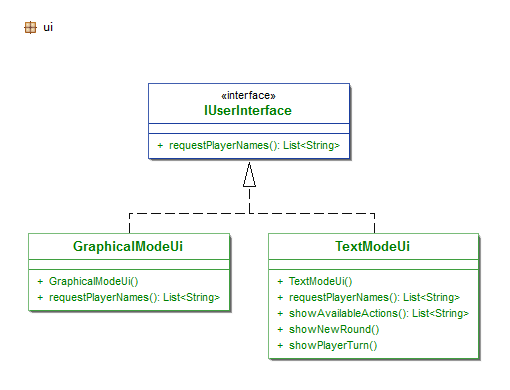
\includegraphics[width=500px]{design-uml/package-ui.png}
        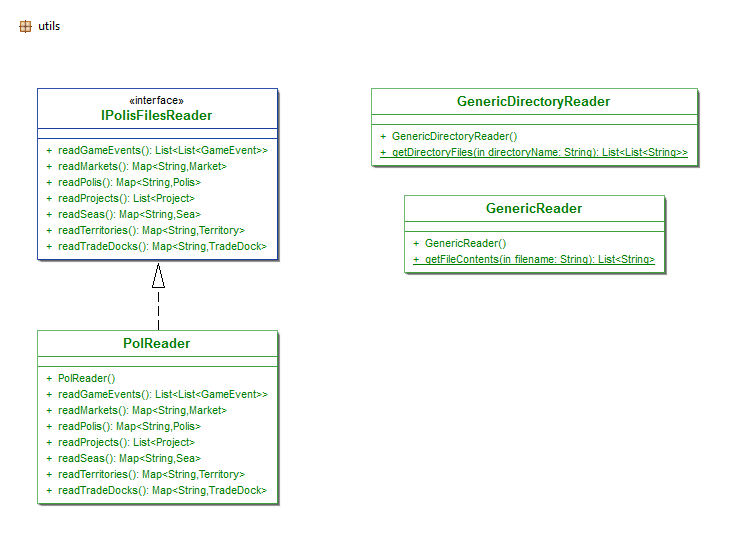
\includegraphics[width=500px]{design-uml/package-utils.png}
    \end{center}
\end{document}

